
\chapter{\elemMatDetIITitle}\label{elementarydeterminantsII}

In section~\ref{elementarydeterminants}, we saw the definition of the determinant and derived an elementary matrix that exchanges two rows of a matrix.  Next, we need to find elementary matrices corresponding to the other two row operations; multiplying a row by a scalar, and adding a multiple of one row to another.  As a consequence, we will derive some important properties of the determinant.

Consider $M=\colvec{R^1 \\ \vdots \\ R^n }$, where $R^i$ are row vectors.  Let $R^i(\lambda)$ be the identity matrix, with the $i$th diagonal entry replaced by $\lambda$, not to be confused with the row vectors. {\it I.e.}
$$
R^i(\lambda)=
\begin{pmatrix}
1 & & & & \\
  & \ddots & & & \\
  & & \lambda & & \\
  & & & \ddots & \\
  & & & & 1 \\
\end{pmatrix}
\, .$$
Then:

\[
M'=R^i(\lambda)M=\colvec{R^1 \\ \vdots \\ \lambda R^i \\ \vdots \\ R^n }
\]
What effect does multiplication by $R^i(\lambda)$ have on the determinant?

\begin{eqnarray*}
\det M' & = & \sum_{\sigma} \text{sgn}(\sigma) m^1_{\sigma(1)}\cdots \lambda m^i_{\sigma(i)} \cdots m^n_{\sigma(n)} \\
& = & \lambda \sum_{\sigma} \text{sgn}(\sigma) m^1_{\sigma(1)}\cdots m^i_{\sigma(i)} \cdots m^n_{\sigma(n)} \\
& = & \lambda \det M
\end{eqnarray*}
Thus, multiplying a row by $\lambda$ multiplies the determinant by $\lambda$.
{\it I.e.,} $$\det R^i(\lambda) M = \lambda \det M\, .$$


\begin{figure}
\begin{center}
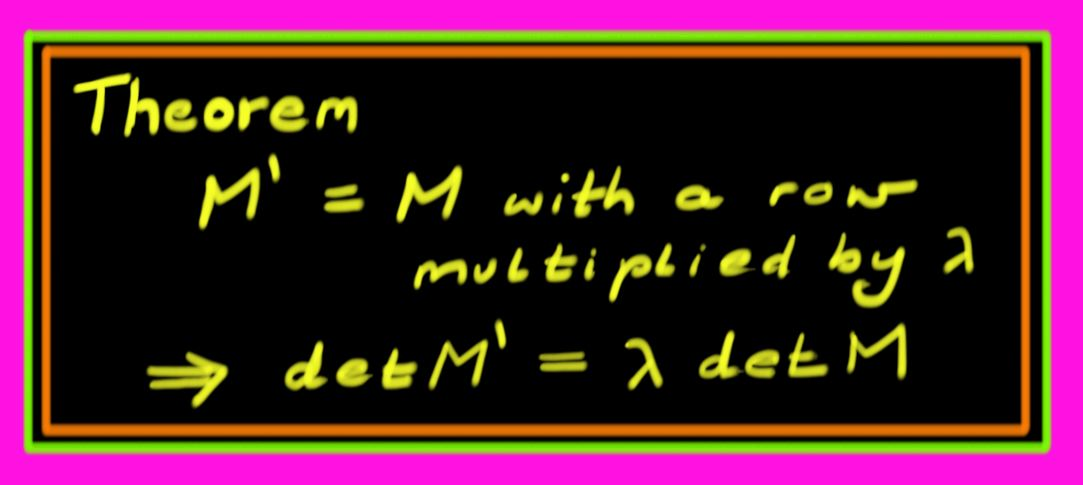
\includegraphics[scale=.27]{\elemMatDetIIPath/row_mult_thm.jpg}
\end{center}
\end{figure}


Since $R^i(\lambda)$ is just the identity matrix with a single row multiplied by $\lambda$, then by the above rule, the determinant of $R^i(\lambda)$ is $\lambda$.  Thus:

\[
\det R^i(\lambda) = \det \begin{pmatrix}
1 & & & & \\
  & \ddots & & & \\
  & & \lambda & & \\
  & & & \ddots & \\
  & & & & 1 \\
\end{pmatrix} = \lambda
\]

The final row operation is adding $\lambda R^j$ to $R^i$.  This is done with the matrix~$S^i_j(\lambda)$, which is an identity matrix but with a $\lambda$ in the $i,j$ position.

\[
S^i_j(\lambda) = \begin{pmatrix}
1 & 	& 	& 	& & & 	\\
  & \ddots & 	&	& & &	\\
  & 	& 1 	& 	& \lambda & &	\\
  & 	& 	& \ddots & & &	\\
  & 	& 	& 	& 1 & & 	\\
  & 	& 	& 	& 	& \ddots & 	\\
  & 	& 	& 	& 	& 	 & 1	\\
\end{pmatrix}
\]
Then multiplying $S^i_j(\lambda)$ by $M$ gives the following:

\[
\begin{pmatrix}
1 & 	& 	& 	& & & 	\\
  & \ddots & 	&	& & &	\\
  & 	& 1 	& 	& \lambda & &	\\
  & 	& 	& \ddots & & &	\\
  & 	& 	& 	& 1 & & 	\\
  & 	& 	& 	& 	& \ddots & 	\\
  & 	& 	& 	& 	& 	 & 1	\\
\end{pmatrix}\colvec{\\ \vdots \\ R^i \\ \vdots \\ R^j \\ \vdots\\ \\}
=
\colvec{\\ \vdots \\ R^i +\lambda R^j \\ \vdots \\ R^j \\ \vdots\\ \\ }
\]
What is the effect of multiplying by $S^i_j(\lambda)$ on the determinant?  Let $M'=S^i_j(\lambda)M$, and let $M''$ be the matrix $M$ but with $R^i$ replaced by $R^j$.

\begin{eqnarray*}
\det M' & = & \sum_{\sigma} \text{sgn}(\sigma) m^1_{\sigma(1)}\cdots (m^i_{\sigma(i)}+ \lambda m^j_{\sigma(j)}) \cdots m^n_{\sigma(n)} \\
& = & \sum_{\sigma} \text{sgn}(\sigma) m^1_{\sigma(1)}\cdots m^i_{\sigma(i)} \cdots m^n_{\sigma(n)} \\
&   & \qquad + \sum_{\sigma} \text{sgn}(\sigma) m^1_{\sigma(1)}\cdots \lambda m^j_{\sigma(j)} \cdots m^j_{\sigma(j)} \cdots m^n_{\sigma(n)} \\
& = & \det M + \lambda \det M''
\end{eqnarray*}
Since $M''$ has two identical rows, its determinant is $0$.  Then $$\det S^i_j(\lambda)M = \det M\, .$$
Notice that if $M$ is the identity matrix, then we have $$\det S^i_j(\lambda) = \det (S^i_j(\lambda)I) = \det I = 1\, .$$

\begin{figure}
\begin{center}
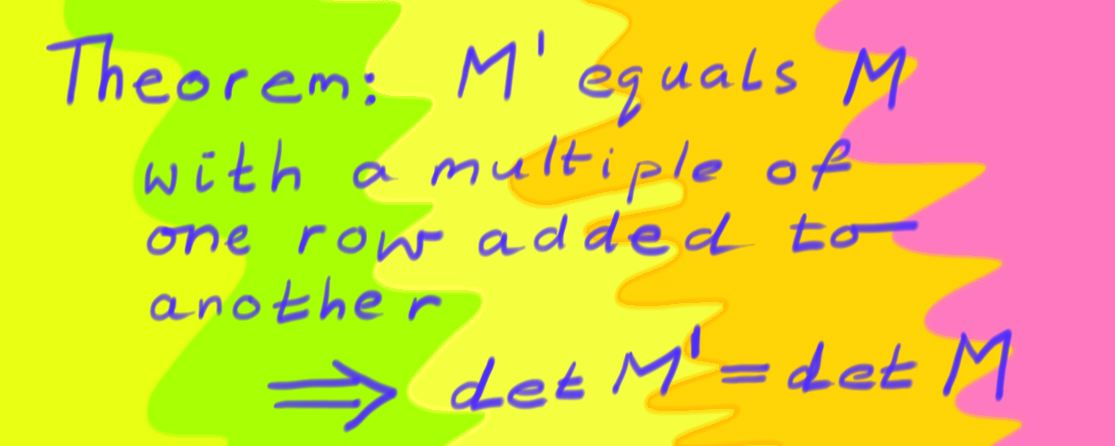
\includegraphics[scale=.27]{\elemMatDetIIPath/row_addition_thm.jpg}
\end{center}
\end{figure}

We now have elementary matrices associated to each of the row operations.

\[
\begin{array}{cccc}
E^i_j &=& I \text{ with rows $i,j$ swapped;} &\det E^i_j=-1 \\[3mm]
R^i(\lambda) &=& I \text{ with $\lambda$ in position $i,i$;} 
	&\det R^i(\lambda)=\lambda \\[3mm]
S^i_j(\lambda) &=& I \text{ with $\lambda$ in position $i,j$;} 
	&\det S^i_j(\lambda)=1 \\[3mm]
\end{array}
\]
\videoscriptlink{elementary_matrices_and_determinants_ii_dets.mp4}{Elementary Determinants}{scripts_elementary_matrices_determinants_ii_dets}
We have also proved the following theorem along the way:

\begin{theorem}
If $E$ is \emph{any} of the elementary matrices $E^i_j, R^i(\lambda), S^i_j(\lambda)$, then $\det(EM)=\det E \det M$.
\end{theorem}

%\href{\webworkurl ReadingHomework13/1/}{Reading homework: problem 13.1}
\reading{13}{1}


\begin{center}
\hspace{3mm}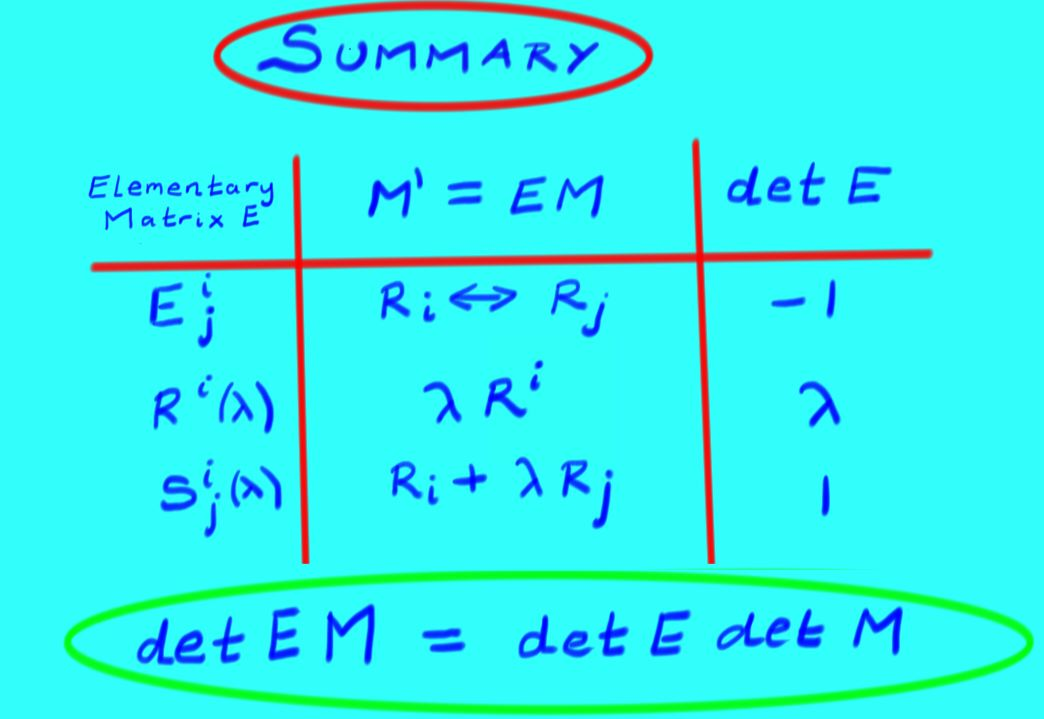
\includegraphics[scale=.27]{\elemMatDetIIPath/summary.jpg}
\end{center}


We have seen that any matrix $M$ can be put into reduced row echelon form via a sequence of row operations, and we have seen that any row operation can be emulated with left matrix multiplication by an elementary matrix.  Suppose that $\rref(M)$ is the reduced row echelon form of $M$.  Then $\rref(M)=E_1E_2\cdots E_kM$ where each $E_i$ is an elementary matrix.

What is the determinant of a square matrix in reduced row echelon form?  
\begin{itemize}
\item If $M$ is not invertible, then some row of $\rref(M)$ contains only zeros.  Then we can multiply the zero row by any constant $\lambda$ without changing~$M$; by our previous observation, this scales the determinant of $M$ by $\lambda$.  Thus, if $M$ is not invertible, $\det \rref(M)=\lambda \det \rref(M)$, and so $\det \rref(M)=0$.  

\item Otherwise, every row of $\rref(M)$ has a pivot on the diagonal; since $M$ is square, this means that $\rref(M)$ is the identity matrix.  Then if $M$ is invertible, $\det \rref(M)=1$.

\item Additionally, notice that $\det \rref(M) = \det (E_1E_2\cdots E_kM)$.  Then by the theorem above, $\det \rref(M)=\det (E_1) \cdots \det (E_k) \det M$.  Since each $E_i$ has non-zero determinant, then $\det \rref(M)=0$ if and only if $\det M=0$.
\end{itemize}
Then we have shown:

\begin{theorem}
\label{detinvertible}
For any square matrix $M$, $\det M\neq 0$ if and only if $M$ is invertible.
\end{theorem}
Since we know the determinants of the elementary matrices, we can immediately obtain the following:


\videoscriptlink{elementary_matrices_ii_inverses_determinants.mp4}{Determinants and Inverses}{scripts_elementary_matrices_determinants_ii_inverses}

\begin{figure}
\begin{center}
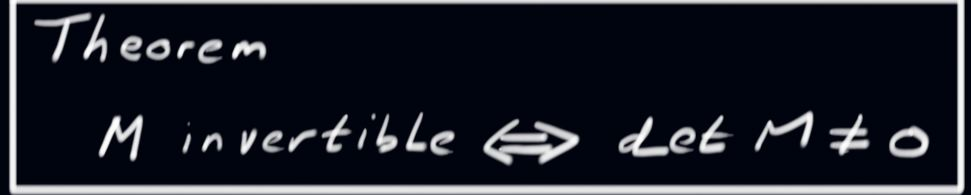
\includegraphics[scale=.27]{\elemMatDetIIPath/theorem_invertible.jpg}
\end{center}
\end{figure}

\begin{corollary}
Any elementary matrix $E^i_j, R^i(\lambda), S^i_j(\lambda)$ is invertible, except for $R^i(0)$.  In fact, the inverse of an elementary matrix is another elementary matrix.
\end{corollary}


To obtain one last important result, suppose that $M$ and $N$ are square $n\times n$ matrices, with reduced row echelon forms such that, for elementary matrices  $E_i$ and $F_i$, $$M=E_1E_2\cdots E_k \, \rref(M)\, ,$$ and  $$N=F_1F_2\cdots F_l \, \rref(N)\, .$$  If $\rref(M)$ is the identity matrix ({\it i.e.}, $M$ is invertible), then:

\begin{eqnarray*}
\det (MN) & = & \det (E_1E_2\cdots E_k\,  \rref(M) F_1F_2\cdots F_l \, \rref(N) )\\
& = & \det (E_1E_2\cdots E_k I F_1F_2\cdots F_l\,  \rref(N) )\\
& = & \det (E_1) \cdots \det(E_k)\det(I)\det(F_1)\cdots\det(F_l)\det(\rref(N)\\
& = & \det(M)\det(N)
\end{eqnarray*}
Otherwise, $M$ is not invertible, and $\det M=0=\det 
\rref(M)$.  Then there exists a row of zeros in $
\rref(M)$, so $R^n(\lambda)
\rref(M)=
\rref(M)$.  Then:
\begin{eqnarray*}
\det (MN) & = & \det (E_1E_2\cdots E_k 
\, \rref(M) N )\\
& = & \det (E_1E_2\cdots E_k 
\, \rref(M) N )\\
& = & \det (E_1) \cdots \det(E_k)\det( 
\rref(M)N)\\
& = & \det (E_1) \cdots \det(E_k)\det( R^n(\lambda) 
\, \rref(M)N)\\
& = & \det (E_1) \cdots \det(E_k)\lambda \det( 
\rref(M)N)\\
& = & \lambda \det (MN)
\end{eqnarray*}
Which implies that $\det (MN)=0=\det M \det N$.

Thus we have shown that for {\it any} matrices $M$ and $N$, 
\label{detmultiplicative}
\[
\det (MN) = \det M \det N
\]
This result is {\it extremely important}; do not forget it!

\videoscriptlink{elementary_matrices_determinant_ii_product.mp4}{Alternative proof}{scripts_elementary_matrices_determinants_ii_product}

\begin{figure}
\begin{center}

\includegraphics[scale=.27]{\elemMatDetIIPath/detMN.jpg}
\end{center}
\end{figure}

%\href{\webworkurl ReadingHomework13/2/}{Reading homework: problem 13.2}
\reading{13}{2}

%\section*{References}
%Hefferon, Chapter Four, Section I.1 and I.3
%\\
%Beezer, Chapter D, Section DM, Subsection EM
%\\
%Beezer, Chapter D, Section PDM
%\\
%Wikipedia:
%\begin{itemize}
%\item \href{http://en.wikipedia.org/wiki/Determinant}{Determinant}
%\item \href{http://en.wikipedia.org/wiki/Elementary_matrix}{Elementary Matrix}
%\end{itemize}

\section{Review Problems}




\begin{enumerate}

\item While performing  Gaussian elimination on these augmented matrices write the full system of equations describing the new rows in terms of the old rows above each equivalence symbol as in  \hyperlink{Keeping track of EROs with equations between rows}{Example}~\ref{Rsystem}. 
$$
\begin{amatrix}{2} 
2 & 2 & 10 \\
1 & 2 & 8 \\
\end{amatrix}
,~
\begin{amatrix}{3} 
1 & 1 & 0 & 5 \\
1 & 1 & \!\!-1& 11 \\
-1 & 1 & 1 & -5 \\ 
\end{amatrix}
$$

%%%%%%%%%%%%%%%%%%%

\item Solve the vector equation by applying ERO matrices to each side of the equation to perform elimination. Show each matrix explicitly as in \hyperlink{Undoing}{Example~\ref{slowly}}.

\begin{eqnarray*}
\begin{pmatrix}
3	&6 	&2 \\ %-3
5 	&9 	&4 \\ %1
2	&4	&2 \\ %0
\end{pmatrix} 
\begin{pmatrix}
 x \\ 
y \\
z 
\end{pmatrix} 
=
\begin{pmatrix}
-3 \\ 
1  \\
0  \\
\end{pmatrix} 
\end{eqnarray*}

%%%%%%%%%%%%%%%%%%%

\item Solve this vector equation by finding the inverse of the matrix through $(M|I)\sim (I|M^{-1})$ and then applying $M^{-1}$ to both sides of the equation. 
\begin{eqnarray*}
\begin{pmatrix}
2	&1 	&1 \\ %9
1 	&1 	&1 \\ %6
1	&1	&2 \\ %7
\end{pmatrix} 
\begin{pmatrix}
 x \\ 
y \\
z 
\end{pmatrix} 
=
\begin{pmatrix}
9 \\ 
6  \\
7  \\
\end{pmatrix} 
\end{eqnarray*}


%%%%%%%%%%%%%%%%%%%

\item Follow the method of  \hyperlink{elldeeeww}{Examples~\ref{factorize} and~\ref{factorizes}} to find the $LU$ and $LDU$ factorization of 
\begin{eqnarray*}
\begin{pmatrix}
3	&3 	&6 \\ %0 %2
3 	&5 	&2 \\ %1 %1
6	&2	&5 \\ %0 %1
\end{pmatrix} .
\end{eqnarray*}



%%%%%%%%%%%%%%%%%%%%

\item 
Multiple matrix equations with the same matrix can be solved simultaneously. 
\begin{enumerate}
\item Solve both systems by performing elimination on just one augmented matrix.
\begin{eqnarray*}
\begin{pmatrix}
2	&-1 	&-1 \\ %0 %2
-1 	&1 	&1 \\ %1 %1
1	&-1	&0 \\ %0 %1
\end{pmatrix} 
\begin{pmatrix}
 x \\ 
y \\
z 
\end{pmatrix} 
=
\begin{pmatrix}
0\\ 
1  \\
0  \\
\end{pmatrix} 
,~
\begin{pmatrix}
2	&-1 	&-1 \\ %0 %2
-1 	&1 	&1 \\ %1 %1
1	&-1	&0 \\ %0 %1
\end{pmatrix} 
\begin{pmatrix}
 a \\ 
b \\
c 
\end{pmatrix} 
=
\begin{pmatrix}
2\\ 
1  \\
1  \\
\end{pmatrix} 
\end{eqnarray*}
\item Give an interpretation of the columns of $M^{-1}$ in $(M|I)\sim (I|M^{-1})$ in terms of solutions to certain systems of linear equations.
\end{enumerate}

%%%%%%%%%%%%%%%%%%%%%%%%

\item How can you convince your fellow students to never make this mistake?
\begin{eqnarray*}
\begin{amatrix}{3} 
1 & 0 & 2 & 3 \\ 
0 & 1 & 2& 3 \\
2 & 0 & 1 & 4 \\
\end{amatrix} 
& 
\stackrel{R_1'=R_1+R_2}{
\stackrel{R_2'=R_1-R_2}{ 
\stackrel{\ R_3'= R_1+2R_2}{\sim}}}
&
\begin{amatrix}{3} 
1 & 1 & 4 & 6 \\
1 & \!\!-1 & 0& 0 \\
1 & 2 & 6 & 9 
\end{amatrix}
\end{eqnarray*}

\item Is $LU$ factorization of a matrix unique?  Justify your answer.


\item[$\infty$.] If you randomly create a matrix by picking numbers out of the blue, it will probably be difficult to perform elimination or factorization; fractions and large numbers will probably be involved. To invent simple problems it is better to start with a simple answer:
\begin{enumerate}
\item Start with any augmented matrix in RREF. Perform EROs to make most of the components non-zero. Write the result on a separate piece of paper and give it to your friend. Ask that friend to find RREF of the augmented matrix you gave them. Make sure they get the same augmented matrix you started with.  
\item Create  an upper triangular matrix $U$ and a lower triangular matrix~$L$ with only $1$s on the diagonal. Give the result to a friend to factor into $LU$ form. 
\item Do the same with an $LDU$ factorization. 
\end{enumerate}
\end{enumerate}

\phantomnewpage



\newpage



